\documentclass{article}
\usepackage{amsmath}
\usepackage{amssymb}
\usepackage[dvipsnames]{xcolor}
\usepackage{graphicx}
\usepackage{enumitem}
\usepackage{centernot}
\usepackage[margin=1.2in]{geometry}
\begin{document}

\title{Algorithms Quiz \#3}
\author{Ozaner Hansha}
\date{March 13, 2020}
\maketitle

For the following questions consider the following directed graph:
\begin{center}
  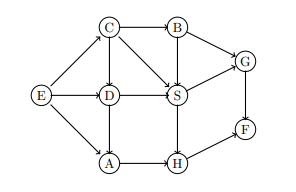
\includegraphics{graph.png}
\end{center}

\subsection*{Part a}
\noindent\textbf{Problem:} Do a DFS starting at $E$, assuming vertices are to be considered in alphabetical order. List each vertex along with their discovery and finish times. Then classify each edge as a tree edge, back edge,
forward edge, or cross edge.
\bigskip

\noindent\textbf{Solution:} The discovery and finish times for each vertex are given below (note that time starts at $t=1$):
\begin{center}
  \begin{tabular}{c|c|c}
        Vertex & Discovery Time & Finished Time \\
        \hline
        $A$ & $2$ & $7$\\
        $B$ & $9$ & $14$\\
        $C$ & $8$ & $17$\\
        $D$ & $15$ & $16$\\
        $E$ & $1$ & $18$\\
        $F$ & $4$ & $5$\\
        $G$ & $10$ & $11$\\
        $H$ & $3$ & $6$\\
        $S$ & $12$ & $13$
  \end{tabular}
\end{center}
\medskip

Each of the graph's edges is classified below:
\begin{center}
  \begin{tabular}{c|c|c|c}
        Tree Edges & Forward Edges & Cross Edges & Backward Edges \\
        \hline
        $(E,A),(A,H),(H,F),$ & $(E,D),(C,S)$ & $(D,S),(S,G),$\\
        $(E,C),(C,B),(B,G),$ & & $(S,H),(D,A),$\\
        $(B,S),(C,D)$ & & $(G,F)$
  \end{tabular}
\end{center}

\subsection*{Part b}
\noindent\textbf{Problem:}  Use the DFS from part a to do a topological sort on this graph. List the vertices on a line in topological sorted order.
\bigskip

\noindent\textbf{Solution:} Recall that performing a topological sort on a DAG, of which the above graph is due to not having any back edges, is equivalent to listing the finish times of of DFS in reverse order. Thus, our topological sort returns the following ordered list of vertices:

$$E,C,D,B,S,G,A,H,F$$

\subsection*{Part c}
\noindent\textbf{Problem:} Suppose now we add a directed edge from $F$ to $E$ to the graph. Identify the strongly connected components in the new graph.
\bigskip

\noindent\textbf{Solution:} After adding the edge $(F,E)$, the graph itself is strongly connected. Since the set of SCCs partitions the graph, the entire graph must be the only strongly connected component.
\end{document}